\documentclass[11pt,a4paper,notitlepage]{article}

\usepackage[T1]{fontenc}
\usepackage[utf8]{inputenc}
\usepackage[english]{babel}
\usepackage{fullpage}
\usepackage{amsmath}
\usepackage{amsfonts}
\usepackage{amssymb}
\usepackage{verbatim}
\usepackage{listings}
\usepackage{color}
\usepackage{setspace}
\usepackage{epstopdf}
\usepackage{graphicx}
\usepackage{caption}
\usepackage{subcaption}
\usepackage{float}
\usepackage{epstopdf}
\usepackage{hyperref}
\usepackage{braket}
\pagenumbering{arabic}

\definecolor{codepurple}{rgb}{0.58,0,0.82}
\definecolor{backcolour}{rgb}{0.95,0.95,0.92}
\definecolor{dkgreen}{rgb}{0,0.6,0}
\definecolor{gray}{rgb}{0.5,0.5,0.5}
\definecolor{mauve}{rgb}{0.58,0,0.82}
%\setlength{\parindent}{0pt}

\lstdefinestyle{pystyle}{
  language=Python,
  aboveskip=3mm,
  belowskip=3mm,
  columns=flexible,
  basicstyle={\small\ttfamily},
  backgroundcolor=\color{backcolour},
  commentstyle=\color{dkgreen},
  keywordstyle=\color{magenta},
  numberstyle=\tiny\color{gray},
  stringstyle=\color{codepurple},
  basicstyle=\footnotesize,  
  breakatwhitespace=false
  breaklines=true,
  captionpos=b,
  keepspaces=true,
  numbers=left,
  numbersep=5pt,
  showspaces=false,
  showstringspaces=false,
  showtabs=false,
  tabsize=2
}
\lstdefinestyle{iStyle}{
  language=IDL,
  aboveskip=3mm,
  belowskip=3mm,
  columns=flexible,
  basicstyle={\small\ttfamily},
  backgroundcolor=\color{backcolour},
  commentstyle=\color{dkgreen},
  keywordstyle=\color{magenta},
  numberstyle=\tiny\color{gray},
  stringstyle=\color{codepurple},
  basicstyle=\footnotesize,  
  breakatwhitespace=false
  breaklines=true,
  captionpos=b,
  keepspaces=true,
  numbers=left,
  numbersep=5pt,
  showspaces=false,
  showstringspaces=false,
  showtabs=false,
  tabsize=2
}
\lstdefinestyle{c++style}{
  language=C++,
  keywordstyle=\color{blue}\ttfamily,
  stringstyle=\color{red}\ttfamily,
  commentstyle=\color{green}\ttfamily,
  morecomment=[l][\color{magenta}]{\#}
  aboveskip=3mm,
  belowskip=3mm,
  columns=flexible,
  basicstyle={\small\ttfamily},
  backgroundcolor=\color{backcolour},
  numberstyle=\tiny\color{gray},
  basicstyle=\footnotesize,  
  breakatwhitespace=false
  breaklines=true,
  captionpos=b,
  keepspaces=true,
  numbers=left,
  numbersep=5pt,
  showspaces=false,
  showstringspaces=false,
  showtabs=false,
  tabsize=2
}

\title{\normalsize Fys4150: Computational Physics \\
\vspace{10mm}
\huge Project 1\\
\vspace{10mm}
\normalsize Due date {\bf 19.th of September, 2016 - 23:59}}

% Skriv namnet ditt her og fjern kommenteringa
\author{Øyvind B. Svendsen, Magnus Christopher Bareid \\ un: oyvinbsv, magnucb}

\newcommand\pd[2]{\frac{\partial #1}{\partial #2}}
\def\doubleunderline#1{\underline{\underline{#1}}}


\begin{document}
\noindent
\maketitle
\vspace{10mm}
\begin{abstract}
The aim of this project is to get familiar with various vector and matrix operations, from dynamic memory allocation to the usage of programs in the library package of the course.

The student was invited to use either brute force-algorithms to calculate linear algebra, or to use a set of recommended linear algebra packages through Armadillo that simplify the syntax of linear algebra. Additionally, dynamic memory handling is expected.

The students will showcase necessary algebra to perform the tasks given to them, and explain the way said algebra is implemented into algorithms. In essence, we're asked to simplify a linear second-order differential equation from the form of the Poisson equation, seen as
\begin{align*}
\nabla ^2 \Phi = -4\pi\rho(\mathbf{r})
\end{align*}
into a one-dimensional form bounded by Dirichlet boundary conditions.
\begin{align*}
-u''(x) = f(x)
\end{align*}
so that discretized linear algebra may be committed unto the equation, yielding a number of numerical methods for aquiring the underivated function $u(x)$.
\end{abstract}
\begin{center}
\line(1,0){450}
\end{center}

%\newpage
\tableofcontents

\newpage
\section{Introduction}
The production of this document will inevitably familiarize its authors with the programming language \verb|C++|, and to this end mathematical groundwork must first be elaborated to translate a Poisson equation from continuous calculus form, into a discretized numerical form.

The Poisson equation is rewritten to a simplified form, for which a real solution is given, with which we will compare our numerical approximation to the real solution.

\section{Problem}
%something something dark side about how we decompose the abstract problem into a real programmable problem

\section{Method}


\label{section:method}
Reviewing the Poisson equation:
\begin{align*}
\nabla ^2 \Phi &= -4\pi\rho(\mathbf{r}), \ \text{which is simplified one-dimensionally by} \ \Phi(r) = \phi(r)/r \\
\Rightarrow \frac{d^2 \phi}{dr^2} &= -4\pi r \rho(r), \ \text{which is further simplified by these substitutions:}\\
r &\rightarrow x, \\
\phi &\rightarrow u,\\
4\pi r\rho(r) &\rightarrow f, \indent \text{which produces the simplified form}
\end{align*}\begin{align*}\label{eq:1}\tag{1}
-u''(x) &= f(x), \indent \text{for which we assume that} \indent f(x) = 100e^{-10x}, \\
\Rightarrow u(x) &= 1- (1-e^{-10})x - e^{-10x},\ \text{with bounds:}\ x \in [0,1],\ u(0) = u(1)= 0
\end{align*}
From here on and out, the methods for finding $u(x)$ numerically will be deduced.

To more easily comprehend the syntax from a programming viewpoint, one may refer to the each discretized representation of $x$ and $u$; we know the span of $x$, and therefore we may divide it up into appropriate chunks. Each of these $x_i$ will yield a corresponding $u_i$.

We may calculate each discrete $x_i$ by the form $x_i = ih$ in the interval from $x_0 = 0$ to $x_{n} = 1$ as it is linearly increasing, meaning we use $n$ points in our approximation, yielding the step length $h = 1/n$. Of course, this also yields discretized representation of $u(x_i) = u_i$.

Through Euler's teachings on discretized numerical derivation methods, a second derivative may be constructed through the form of
\begin{align}
\nonumber
\left(\pd{u}{x}\right)_{fw} = \frac{u_{i+1} - u_i}{h} \quad\quad
\left(\pd{u}{x}\right)_{bw} = \frac{u_{i} - u_{i-1}}{h} \\
\nonumber
\left(\pd{}{x}\right)^2[u_i] = \left(\pd{}{x}_{bw}\right)\left(\pd{}{x}\right)_{fw}[u_i] = \left(\pd{}{x}\right)_{bw}\left(\frac{u_{i+1} - u_i}{h}\right) =\frac{\left(\pd{u_{i+1}}{x}\right)_{bw} - \left(\pd{u_i}{x}\right)_{bw}}{h} \\
\nonumber
\left(\pd{}{x}\right)^2[u_i] = \frac{u_{+1} - 2u_i + u_{i-1}}{h^2}\\
\label{eq:2} \tag{2}
-u''(x) = - \frac{u_{i+1} - 2u_i + u_{i-1}}{h^2} = \frac{- u_{i+1} + 2u_i - u_{i-1}}{h^2} = f_i , \indent \text{for}\ i = 1, \hdots, n
\end{align}

%TODO Bareid, look at this
The discretized prolem can now be solved as a linear algebraic problem.
Looking closer at the discretized problem:
\begin{align*}
	-u''(x_i) = \frac{- u_{i+1} + 2u_i - u_{i-1}}{h^2} &= f_i \\
	\Rightarrow -u_{i+1} + 2u_i - u_{i-1} &= h^2f_i = y_i\\
	i = 1: \quad -u_2 + 2u_1 - u_0 &= y_1 \\
	i = 2: \quad -u_3 + 2u_2 - u_1 &= y_2 \\
	i = 3: \quad -u_4 + 2u_3 - u_2 &= y_3 \\
	\vdots& \\
	i = n: \quad -u_{n+1} + 2u_n - u_{n-1} &= y_n \\
	\intertext{This is very similar to a linear algebra /matrix problem and we will test a system of equations to match.}
	A \vec{u} &= \vec{y} \\
	\begin{bmatrix} %matrix A
		2 & -1 & 0 & \hdots & \\
		-1 & 2 & -1 & \hdots & \\
		0 & -1 & 2 & \ddots & \\
		\vdots & \vdots & \ddots & \ddots & \\
		& & & & 
	\end{bmatrix} %matrix A
	\begin{bmatrix} %vector u
		u_0 \\
		u_1 \\
		\vdots \\
		\\
		u_{n+1}
	\end{bmatrix} %vector u
	&= \begin{bmatrix} %vector y
		y_0 \\
		y_1 \\
		\vdots \\
		\\
		y_{n+1}
	\end{bmatrix} %vector u
	\intertext{This matrix equation will not be valid for the first and last values of $\vec{y}$ because they would require elements of $\vec{u}$ that are not defined; $u_{-1}$ and $u_{n+2}$. Given this constraint we see that the matrix-equation gives the same set of equations that we require.}
	i = 1: \quad -u_2 + 2u_1 - u_0 &= y_1 \\
	i = 2: \quad -u_3 + 2u_2 - u_1 &= y_2 \\
	i = 3: \quad -u_4 + 2u_3 - u_2 &= y_3 \\
	\vdots& \\
	i = n: \quad -u_{n+1} + 2u_n - u_{n-1} &= y_n
\end{align*}
%END TODO

The coefficients from each of these terms and their corresponding value of $u(x)$ may be represented by a tridiagonal matrix multiplication:
\begin{align*}
-\frac{d^2}{dx^2}u(x) = f(x) \indent \Rightarrow \indent \mathbf{\hat{A}}\mathbf{\hat{u}} = h^2\mathbf{\hat{f}} \indent \Rightarrow \indent \left(\begin{matrix}
  2     & -1     & 0      & \dots  & \dots  & 0      \\
 -1     &  2     & -1     & 0      &        & \vdots \\
  0     & -1     &  2     & \ddots & \ddots & \vdots \\
 \vdots & 0      & \ddots & \ddots & \ddots & 0      \\
 \vdots &        & \ddots & \ddots & \ddots & -1     \\
  0     & \dots  & \dots  & 0      & -1     & 2      \\
\end{matrix}\right) \left(\begin{matrix}
u_0 \\
\vdots\\
\vdots\\
\vdots\\
\vdots\\
u_n \\
\end{matrix}\right) = h^2\left(\begin{matrix}
f_0 \\
\vdots\\
\vdots\\
\vdots\\
\vdots\\
f_n \\
\end{matrix}\right)
\end{align*}
The double derivation is now reduced to a discretized linear algebra  operation by way of matrix multiplication. In our case, $f(x)$ is known to us, and the only unknowns are the $u(x)$'s from $u_1 \rightarrow u_{n-1}$, as per the Dirichlet boundary conditions, which allows the use of the algorithm from equation \href{eq:2}.

%TODO My stuff
The original problem at hand (the Poisson equation) has now been "degraded" to a simpler, linear algebra problem. \\
Solving a tridiagonal matrix-problem like this is done by gaussian elimination of the tridiagonal matrix A, and thereby solving $\vec{u}$ for the resulting diagonal-matrix. \\

Firstly the tridiagonal matrix A is rewritten to a series of three vectors $\vec{a}$, $\vec{b}$, and $\vec{c}$ that will represent a general tridiagonal matrix. This will make it easier to include other problems of a general form later. \\
The tridiagonal matrix A (with the vector y) now looks like: 
\begin{align*}
	\begin{bmatrix} %matrix [Ay]
		b_1 & c_1 & 0 & 0 & \hdots && y_1\\
		a_2 & b_2 & c_2 & 0 &&& y_2\\
		0 & a_3 & b_3 & c_3 &&& \vdots\\
		0 & 0 & a_4 & b_4 & \ddots &  & \\
		\vdots &&& \ddots & \ddots & c_{n-1} & y_{n-1} \\
		&&&& a_n & b_n &y_n
	\end{bmatrix} %matrix [Ay]
\end{align*}

The gaussian elimination can be split into two parts; a forward substitution were the matrix-elements $a_i$ are set to zero, and a backward substituion were the vector-elements $u_i$ are calculated from known values. \\

starting with row 2, a row-operation is performed to maintain the validity of the system. The goal is to remove element $a_2$ from the row. This is done by subtracting row 1 (multiplied with some constant 'k' from row 2. \\
\begin{minipage}{0.5\linewidth}
\begin{align*}
	\begin{bmatrix} %matrix [Ay]
		b_1 & c_1 & 0 & 0 & \hdots && y_1\\
		\tilde{a}_2 & \tilde{b}_2 & \tilde{c}_2 & 0 &&& \tilde{y}_2\\
		0 & a_3 & b_3 & c_3 &&& y_3\\
		0 & 0 & a_4 & b_4 & \ddots && \vdots\\
		\vdots &&& \ddots & \ddots & c_{n-1} & y_{n-1} \\
		&&&& a_n & b_n &y_n
	\end{bmatrix} %matrix [Ay]
\end{align*}
\end{minipage}
\begin{minipage}{0.5\linewidth}
	\begin{align*}
	\tilde{Row_2} = Row_2 - k \times Row_1
	\intertext{where k is determined by $\tilde{a}_2 = 0 \quad \Rightarrow k = \frac{a_2}{b_1}$}
	\tilde{b}_2 = b_2 - \frac{a_2}{b_1} c_1 \\
	\tilde{c}_2 = c_2 - \frac{a_2}{b_1} \times 0 = c_2 \\
	\tilde{y}_2 = y_2 - \frac{a_2}{b_1} y_1
	\end{align*}
\end{minipage} \\

Moving on to row 3, and performing a similar operation: \\

\begin{minipage}{0.5\linewidth}
\begin{align*}
	\begin{bmatrix} %matrix [Ay]
		b_1 & c_1 & 0 & 0 & \hdots && y_1\\
		0 & \tilde{b}_2 & c_2 & 0 &&& \tilde{y}_2\\
		0 & \tilde{a}_3 & \tilde{b}_3 & \tilde{c}_3 &&& \tilde{y}_3\\
		0 & 0 & a_4 & b_4 & \ddots && \vdots\\
		\vdots &&& \ddots & \ddots & c_{n-1} & y_{n-1} \\
		&&&& a_n & b_n &y_n
	\end{bmatrix} %matrix [Ay]
\end{align*}
\end{minipage}
\begin{minipage}{0.5\linewidth}
	\begin{align*}
	\tilde{Row_3} = Row_3 - k \times Row_2
	\intertext{where k is determined by $\tilde{a}_3 = 0 \quad \Rightarrow k = \frac{a_3}{\tilde{b}_2}$}
	\tilde{b}_3 = b_3 - \frac{a_3}{\tilde{b}_2} c_2 \\
	\tilde{c}_3 = c_3 - \frac{a_3}{\tilde{b}_2} \times 0 = c_3 \\
	\tilde{y}_3 = y_3 - \frac{a_3}{\tilde{b}_2} \tilde{y}_2
	\end{align*}
\end{minipage} \\

By repeating this step a pattern emerges, and an algorithm can be found: \\
\begin{align*}
	\tilde{b}_{i+1} = b_{i+1} - \frac{a_{i+1}}{\tilde{b}_i} c_{i} \\
	\tilde{y}_{i+1} = y_{i+1} - \frac{a_{i+1}}{\tilde{b}_i} \tilde{y}_i \\
	i = 1, 2, \dots, n-1
\end{align*}

After this procedure, the tridiagonal matrix A is transformed into an uppertriangular matrix. This sort of set of equations can be solved for u, since the last equation has one unknown and the other equations has only two unknowns. \\

\begin{minipage}{0.5\linewidth}
\begin{align*}
	\begin{bmatrix} %matrix [Ay]
		b_1 & c_1 & 0 & 0 & \hdots && y_1\\
		0 & \tilde{b}_2 & c_2 & 0 &&& \tilde{y}_2\\
		0 & 0 & \tilde{b}_3 & \tilde{c}_3 &&& \tilde{y}_3\\
		0 & 0 & a_4 & b_4 & \ddots && \vdots\\
		\vdots &&& \ddots & \ddots & c_{n-1} & y_{n-1} \\
		&&&& a_n & b_n &y_n
	\end{bmatrix} %matrix [Ay]
\end{align*}
\end{minipage}

\section{Explanation of programs}
\subsection{main.cpp}
	The main-program is a \verb|c++|-program designed to take a cmd-line argument that decides the size of the array u, and a boolean argument (0 or 1 that decides wether or not the armadillo-function "solve" should be used.
	
	An x-array between 0 and 1 is calculated and the appropriate a,b,c,y-arrays are calcualted as well. For this program the tridiagonal elements are constantly -1, 2 and -1 while y(x) follows the function described in the introduction. \\
	
	If the boolean cmd-line argument is false, then the program will calculate $\vec{u}$ using the general tridiagonal method(explanation below) and store the CPU-time it takes to calculate $\vec{u}$ using this algorithm.
	Next, $\vec{u}$ will be calculated using the specialized tridiagonal method(explanation below) and store the CPU-time it takes to calculate $\vec{u}$ using this algorithm. \\
	Afterwards, since \verb|c++| is terrible at plotting data, all the data (CPU-time of methods, x-arrays, and u-arrays for both methods) are stored in separate files in the data-folder with the csv-format. \\
	
	If the boolean cmd-line argument is true, then the program will calculate $\vec{u}$ using LU-decomposition method in the armadillo-library, measure the CPU-time it takes and store this time in the time-datafile. \\
	
	The function 'write2file' does exactly what the name suggest, 
	write a string to a file. The file-name is a argument to the function and the string is also a argument to the function. 
	It is worth noting that this function will only append to the end of a file so that it does not accidentally destroy lots of data.\\

	The function 'general\_tridiag' solves the equation $A\hat{x} = \hat{y}$ for $\hat{x}$ when A is a tri-diagonal matrix.
	The tridiagonal elements are three arrays of length n that must be given to the function as arguments along with the vector y and the size of the arrays. In figure \ref{code:general_syntax} the syntax for solving $x_i$ is presented, calculating $\tilde{b_i}$ and $\tilde{y_i}$ in the forward substitution, and $u_i$ in backward substitution, according to the algorithm in section \ref{section:method}. \\
	The comments in figure \ref{code:general_syntax} counts the number of floting point operations in each line. This ammounts to $$5 flops\times(n-3)iterations + 4 flops \times (n-2)iterations = (9n - 23) flops $$ This strange number comes from the fact that the program requires n to be at least 3, since the Dirichlet Boundary Conditions are included in the for-loops. (i.e. excluding calculation of the endpoints, leaving them to be zero according to DBC).\\
	
	The function 'specific\_tridiag' is an attempt at optimizing the code in 'general\_tridiag' and lowering the  number of floating point operations per for-loop. This is primarly done by inserting $-1.0$ for every tridiagonal element $a_i$ and $c_i$, and precalculating the diagonal elements $d_i$ using the formula $d_i = \frac{i+1}{i}$. \\ %TODO
	In figure \ref{code:specific_syntax} the algorithm for an optimized, special-case of the tri-diagonal solver is included. The diagonal elements are already calculated, meaning the forward substitution only applies to $\hat{y}$. The comments counts the number of floating point operations in each iteration. $$ 2flops\times(n-3)iterations + 2flops\times(n-2)iterations = (4n - 10)flops$$ The same restraint applies to this calculation, meaning since the algorithm includes the DBC, n must be three or higher to actually compute any values for $\hat{u}$. \\
	The function 'LU-decomp' simply solves the set of equtions by making the matrix A with armadillo-arrays and using the solve function in the armadillo-library. the function returns the CPU-time it takes to calculate $\hat{u}$
	
\begin{figure}
\label{code:general_syntax}
\lstset{style=c++style}
\begin{lstlisting}[frame=single]
t0 = clock();
//forward substitution
for (int i=1; i<=arg_n-3; i++){
    k = arg_a(i+1)/( (double) arg_b(i) ); //1 flop
    arg_b(i+1) -= k*arg_c(i); //2 flops
    arg_y(i+1) -= k*arg_y(i); //2 flops
}
//backward substitution
for (int i=arg_n-2; i>=1; i--){
  	arg_u(i) = (arg_y(i) - arg_u(i+1)*arg_c(i))/( (double) arg_b(i) ); //4 flops
}
t1 = clock();
return (t1 - t0)/((double) CLOCKS_PER_SEC); //measure time of forward and backward substitution
\end{lstlisting}
\caption{The syntax used in the function 'general\_tridiag' where all variables beginning with arg are function arguments.}
\end{figure}
	
\begin{figure}
\label{code:specific_syntax}
\lstset{style=c++style}
\begin{lstlisting}[frame=single]
t0 = clock();
//forward substitution
for (int i=2; i<=arg_n-2; i++){
	arg_y(i) += arg_y(i-1)/d(i-1); //2 flops
}
//backward substition
for (int i=arg_n-2; i>=1; i--){
    arg_u(i) = (arg_y(i) + arg_u(i+1))/d(i); //2 flops
}
t1 = clock();
return (t1 - t0)/((double) CLOCKS_PER_SEC); //measure time of forward and backward substitution
\end{lstlisting}
\caption{The syntax used in the function 'specific\_tridiag' where all variables beginning with arg are function arguments.}
\end{figure}

\subsection{make\_data.py}
	The program performs the experiment(running 'main.cpp') for several values of n. \\
	Firstly it calculates both tridiagonal solvers and LU-decomposition for n = 10,100,1000 in order to compare the CPU-time for the three methods. \\
	Then it chooses a logarithmic scale of n-values between n=10 and n=10'000 in order to produce data-sets for plotting u(x) and $\epsilon$.

\subsection{plot\_stuff.py}
	This program fetches relevant data produced by 'main.cpp'/'make\_data.py' and stores these data as arrays in a nested dictionary. \\
	Three plotting functions are defined for making appropriate plots: \\
	'compare\_methods' plots u(x) against x for both tridiagonal solvers and the exact solution for a specific n. \\
	'compare\_approx\_n' plots u(x) against x for several values of n for one of the tri-diagonal solvers. \\
	'epsilon\_plots' calculates the maximum relative error and makes a log-log-plot against step-length. This done by calculating the maximum difference between $u_{exact}$ and $u_{general}$ for a series of n-values, using this difference to find the relative error $10^\epsilon = \left|\frac{v-u}{u}\right|$ for every n-value. \\
	These functions are called to make the plots in section \ref{section:results}
	
\section{Results}
\label{section:results}
	The data can be found in the data-folder on the github-repository\footnote{see section \ref{section:github}} and all the figures presented in this section can found in the img-folder in the same repository. \\
\subsection{General tridiagonal solver}
	\begin{figure}
		%compare general with exact for n = 10,100,1000	
		%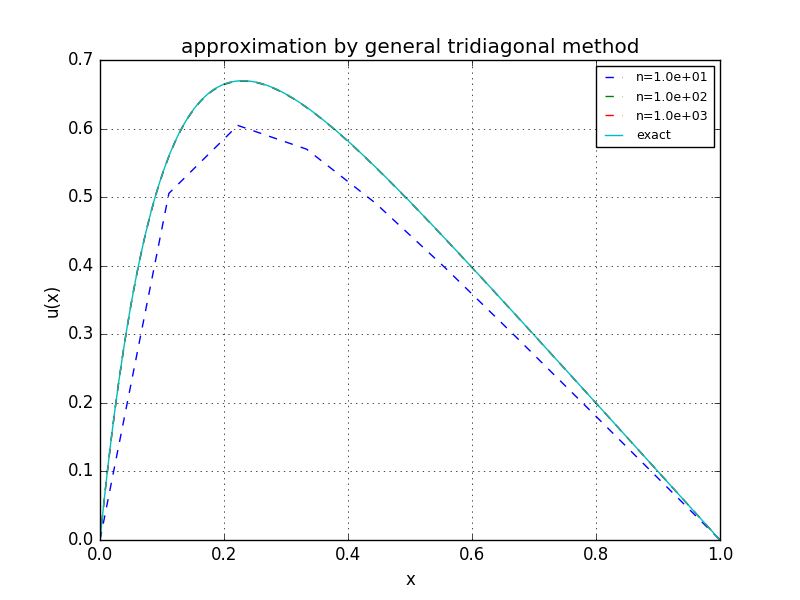
\includegraphics[scale=0.7]{../img/compare_general_exact.png}
		\caption{Compare calculated u(x) with exact solution of u(x) for three values of n, using the general tridiagonal solver.}
		\label{fig:compare_gen_exact}
	\end{figure}

\subsection{CPU-time}
	\begin{table}
		\label{table:cpu-time}
		\begin{align*}
		\begin{tabular}{|c|c|c|c|} \hline
			\log_{10}(n) & general tridiagonal[s] & specific tridiagonal[s] & LU decomposition [s] \\ \hline
			1 & 0.000010 & 0.000006 & 0.008585 \\
			2 & 0.000047 & 0.000007 & 0.015610 \\
			3 & 0.000159 & 0.000123 & 0.699342 \\
			4 & 0.001421 & 0.001749 & \\
			5 & 0.020054 & 0.024508 & \\
			6 & 0.056499 & 0.064189 & \\ \hline
		\end{tabular}
		\end{align*}
		\caption{CPU-time each methods use for calculating u(x) n seconds}
	\end{table}
	
\subsection{Relative error}
	\begin{table}
		\label{table:rel_error}
		\caption{•}
	\end{table}
	\begin{figure}
		\label{fig:rel_error}
		%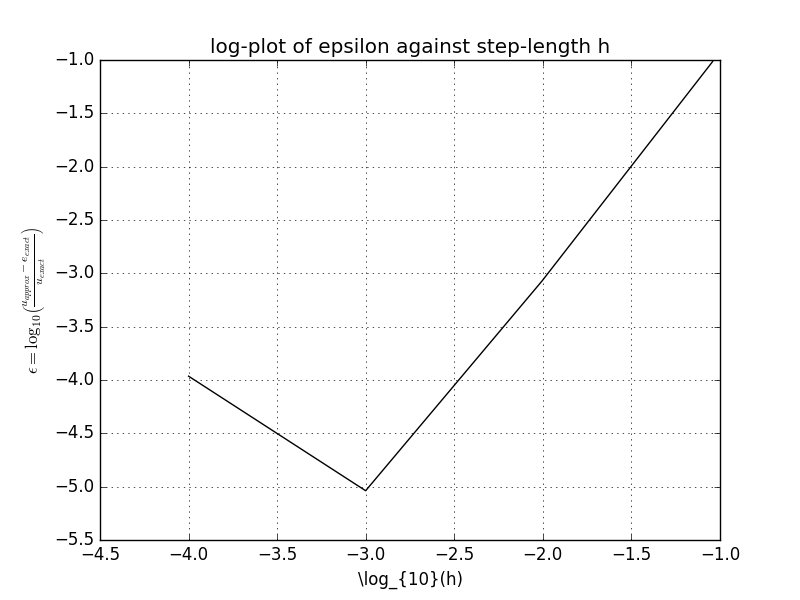
\includegraphics[scale=0.7]{../img/epsilon.png}
		\caption{•}
	\end{figure}
	
\begin{center}
\line(1,0){450}
\end{center}

\newpage
\section{Appendix - Github}
\label{section:github}
This is the code used in this assignment. Anything that was done by hand has been implemented into this pdf, above.
\lstset{style=pystyle}
\verb|plot_stuff.py|
\lstinputlisting{../plot_stuff.py}


\end{document}
